\chapter{Parallel Merging Algorithm}\label{chap:algo}

In \cite{pmalgo}, Siebert et al. proposed a parallel merge algorithm,
in which each processing element will calculate the output range it is
going to produce, and 
use that output range as the input to a \textbf{co-rank function} to identify the corresponding input
ranges that generate the output. Finally, each processing element will call the sequential merge
function to do the merge independently in parallel.

    \section{Co-rank Function}\label{sect:corank}
    Let $A$ and $B$ be two input arrays with $m$ and $n$ elements respectively. Both input arrays 
    are sorted 
    according to an ordering relation $\leq$. The index of the arrays starts from $0$. 
    The task is to merge $A$ and $B$ into an array $C$ with $m+n$ elements. 
    They use $C[m+n] = merge(A[m],B[n],\leq)$ to denote this task.
    In their paper, Siebert et al. pointed out two observations:
    \begin{itemize} 
        \item   For any $i$, $0 \leq i < m+n$ in $C$, there is either a $j$, $0 \leq j < m$ such that 
                $C[i] = A[j]$ or a $k$, $0 \leq k < n$ such that $C[i] = B[k]$. 
        \item   For any $i$-element prefix $C[0,...,i-1]$ of $C$, there must be indices $j$ 
                and $k$ of $A$ and $B$ such that $C[0,...,i-1] = merge(A[0,...,j-1],
                B[0,...,k-1],\leq)$.
    \end{itemize}
    Siebert et al. also proved that $j$ and $k$, which define
    the prefixes of $A$ and $B$ needed to produce the prefix of C of length $i$, are unique. 
    For an element $C[i]$, they call the index $i$ its rank. And they call the unique indices $j$ and $k$ 
    its co-ranks. Consequently, 
    they use the term \textbf{co-rank} for the process of determining $j$ and $k$ from $A, m, B, n$ and $i$.
    Notice that $i = j + k$ because the number of elements in the output array equals the sum of the number of elements
    in the input arrays. 
    Figure \ref{fig:corank} shows an example of co-rank. In this example, $C[16] = merge(A[8],B[8],\leq)$.
    $C[8] = merge(A[5],B[3],\leq)$. Therefore, the co-rank of $8$ is $5$ and $3$.  

    \begin{figure}[!h]
    \begin{center}
    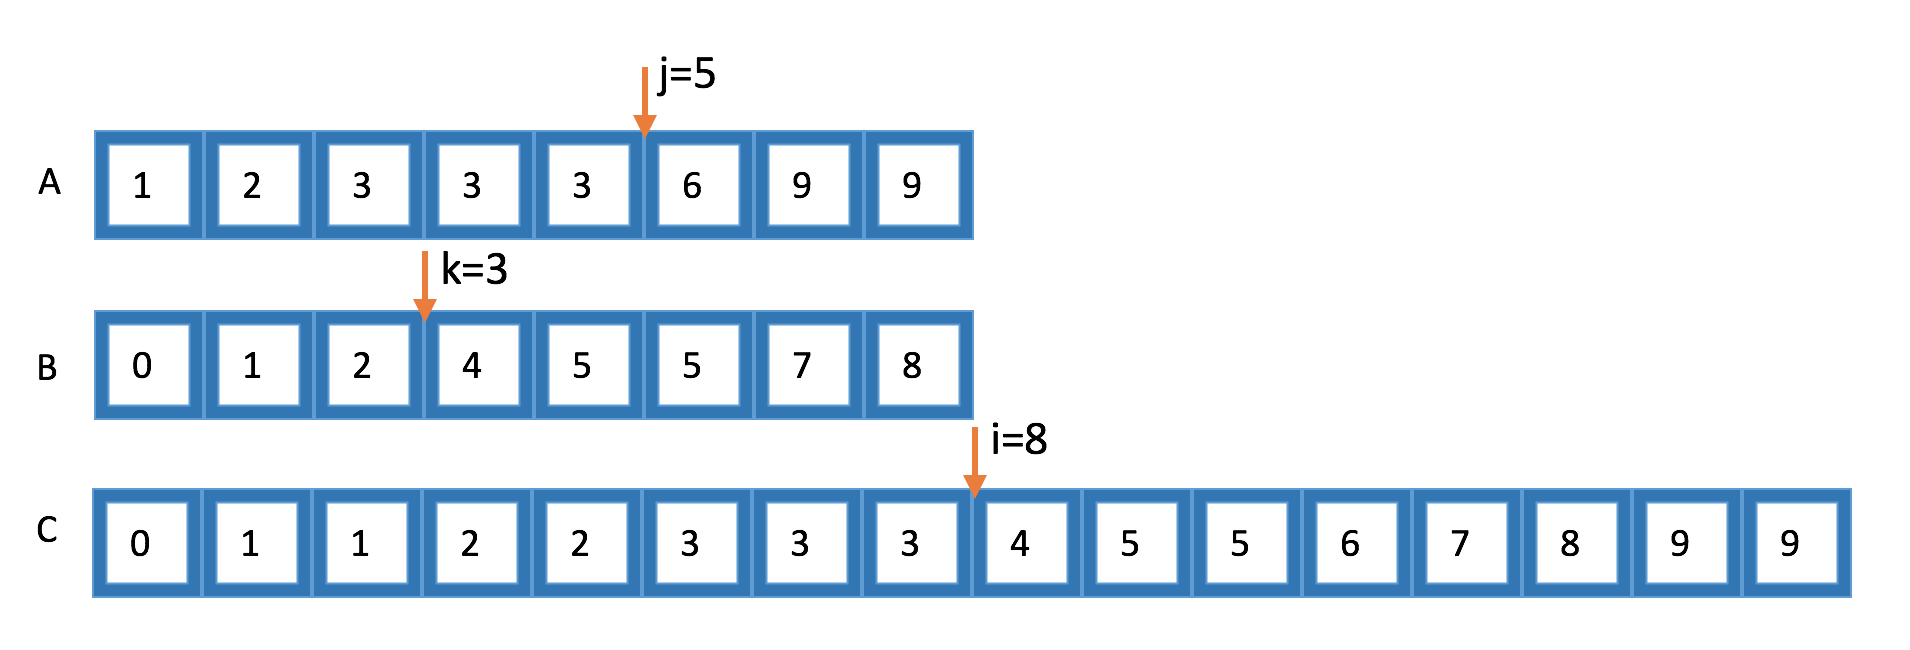
\includegraphics[width=\textwidth]{corank.png}
    \end{center}
    \caption{{\label{fig:corank}} Co-rank Example}
    \end{figure}

    The pseudo code to find the co-rank from $A, m, B, n$ and $i$ is also given in their paper.  
    In listing \ref{list:corank_origin}, we transform their pseudo code into the C++ implementation of 
    co-rank function. We calculate
    $j$ by using $j = co\_rank\_j(i, A, m, B, n)$. Then we calculate $k$ by $k = i - j$.  

    \begin{minipage}{\linewidth}
    \begin{singlespace}
    \begin{lstlisting} [caption = {Original Co-rank}, captionpos=b, label = {list:corank_origin}]
int co_rank_j(int i, int* A, int m, int* B, int n)
{
    int j = i < m ? i : m;                //j = min(i,m)
    int k = i - j;
    int j_low = 0 > (i-n) ? 0 : i-n;      //j_low = max(0, i-n) 
    int k_low;
    int delta;
    bool active = true;

    while(active)
    {
        if (j > 0 && k < n && A[j-1] > B[k]) {
            delta = ((j - j_low - 1) >> 1) + 1;
            k_low = k;
            j = j - delta;
            k = k + delta;
         } else if (k > 0 && j < m && B[k-1] >= A[j]) {
            delta = ((k - k_low - 1) >> 1) + 1;
            j_low = j;
            j = j + delta;
            k = k - delta;
        } else {
            active = false;
        }
    }
    return j;
}
    \end{lstlisting}
    \end{singlespace}
    \end{minipage}

    \section{Overall Parallel Merge}\label{sect:overall}
    The co-rank function provides a simple and efficient way to perform merging in 
    parallel. Let $p$ processing elements be given, all of which can access input and 
    output arrays $A$, $B$ and $C$. Each processing element has its own id $r$, $0 \leq r < p$. 
    
    Each processing element will calculate the output range ($C[i\_start,...i\_end]$) it is 
    going to produce.  
    The output ranges can be chosen such that  
    they cover the whole output array of size $m + n$, and the size of output each processing
    element producing differs by at most $1$. 
    Then, each processing element computes the corresponding co-ranks for both the 
    start and end index. 
    These co-ranks determine the input ranges of the input arrays this processing element needs 
    to merge sequentially.  

    Listing \ref{list:pseudo_merge} shows the pseudo code for the parallel merge algorithm.

    \begin{minipage}{\linewidth}
    \begin{singlespace}
    \begin{lstlisting} [caption = {Pseudo Code for Parallel Merge Algorithm}, captionpos=b, label = {list:pseudo_merge}, mathescape=true]
void paralle_merge(int *A, int m, int *B, int n, int*C) 
{
    r       = processing_id;        // 0 <= r < p
    i_start = floor(r*(m+n)/p);     // start index of output 
    i_end   = floor((r+1)*(m+n)/p); // end   index of output 
    j_start = co_rank_j(i_strat, A, m, B, n);
    j_end   = co_rank_j(i_end,   A, m, B, n);
    k_start = i_start - j_start;
    k_end   = i_end   - j_end;
    merge( A[j_start,...,j_end-1], B[k_start,...,k_end-1],
           C[i_start,...,i_end-1] );
}
    \end{lstlisting}
    \end{singlespace}
    \end{minipage}

    Figure \ref{fig:overall} shows an example of the parallel merge process. In this example,
    there are two processing elements($p=2$). These two processing elements are going to do 
    the task $C[16] = merge(A[8],B[8],\leq)$ collaboratively in parallel. 

    \begin{figure}[!h]
    \begin{center}
    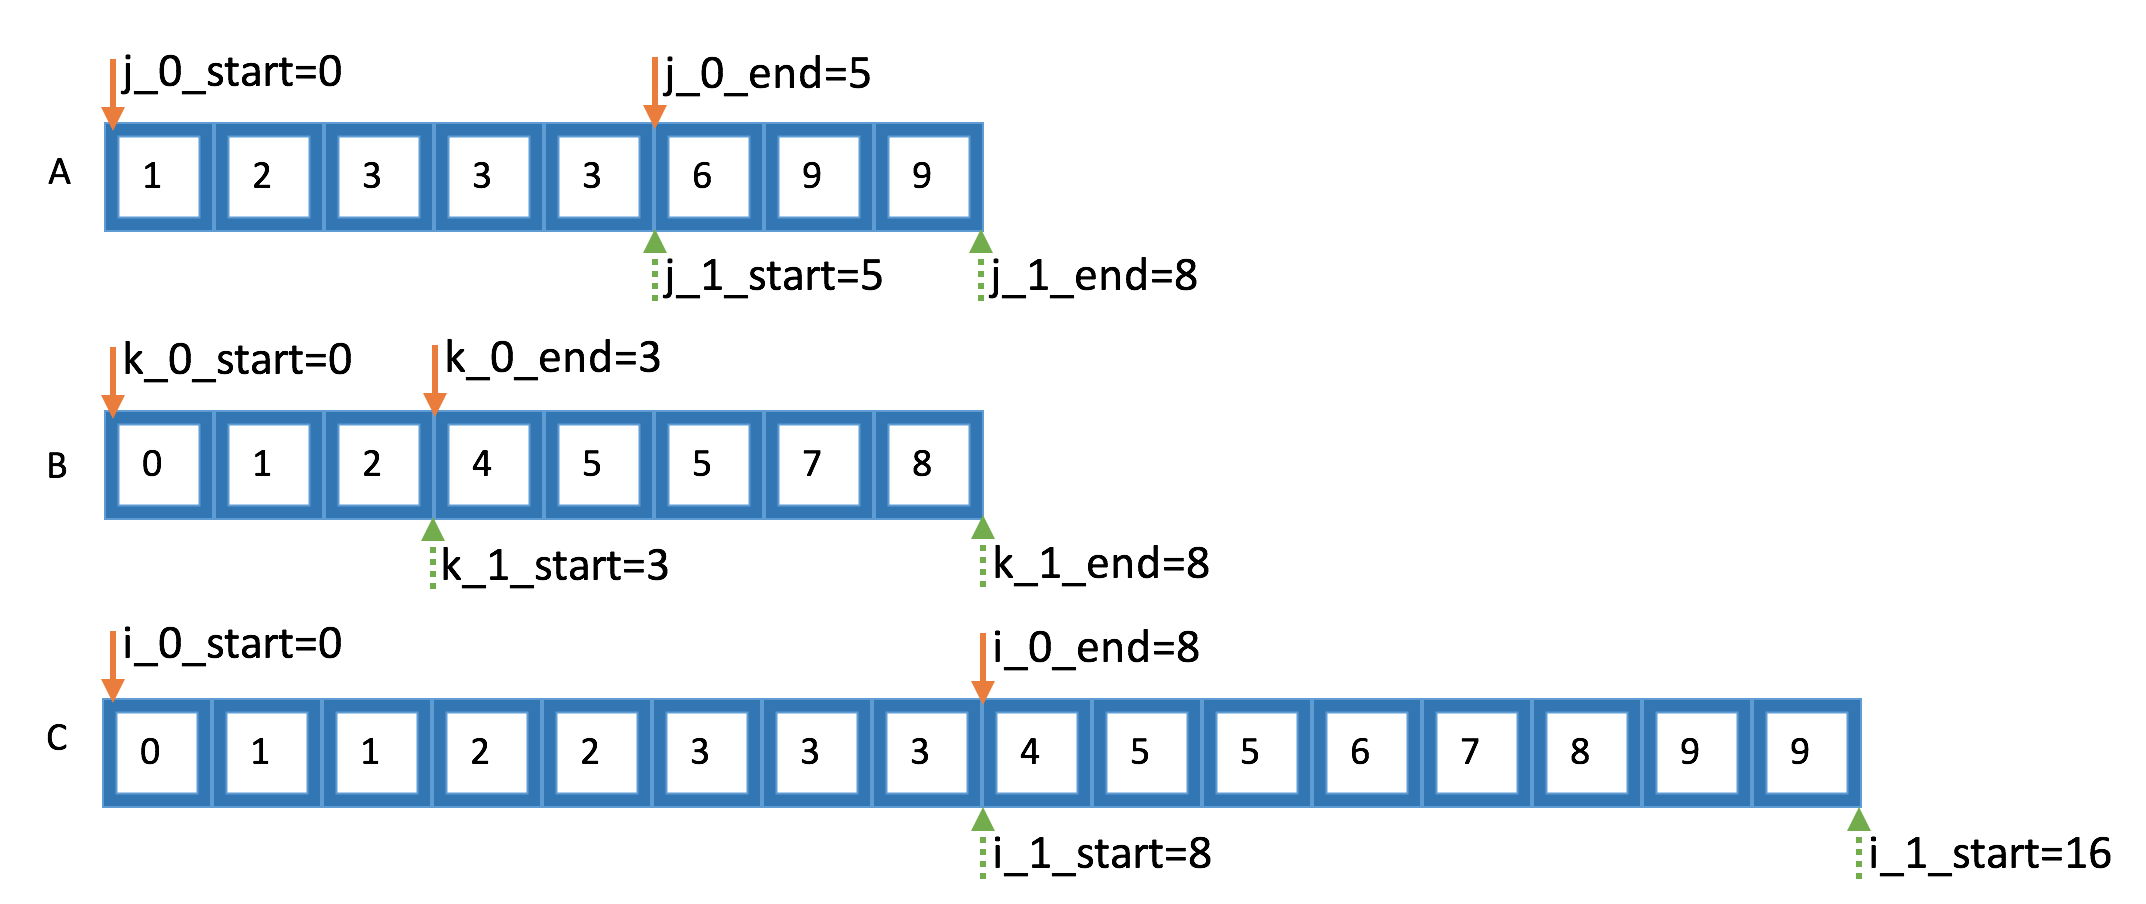
\includegraphics[width=\textwidth]{overall.png}
    \end{center}
    \caption{{\label{fig:overall}} Parallel Merge Algorithm Example}
    \end{figure}   
 
    For $p_0$ (solid red arrows), $r = 0$, $i\_start = 0$, $i\_end=8$. It is going to produce
    $C[0,...,7]$. After running the co-rank function, $p_0$ knows the input ranges: $j\_start = 0$, 
    $j\_end=5$, $k\_start = 0$, $k\_end=3$. Therefore, $p_0$ will call 
    $C[0,...,7] = merge(A[0,...,4],B[0,...,2],\leq)$.

    For $p_1$ (dashed green arrows), $r = 1$, $i\_start = 8$, $i\_end=16$. It is going to produce
    $C[8,...,15]$. After running the co-rank function, $p_1$ knows: $j\_start = 5$, 
    $j\_end=8$, $k\_start = 3$, $k\_end=8$. So $p_1$ will call 
    $C[8,...,15] = merge( A[5,...,7],B[3,...,7],\leq)$.

    Because $p_0$ and $p_1$ are working on different parts of the input and output, they can run in 
    parallel without interference. Also, the sizes of output they produce are the same. 
    Therefore, load balance is guaranteed.      



    % \section{Stable Merge}\label{sect:stable}
    % This subsection will discuss the property of stable merge.

    \section{Implementation on CPU}\label{sect:CPU}
    We implement the parallel merge algorithm on CMPs using openMP. 
    The CPU we are using has 8 threads. Each thread first calculates the output 
    range it is going to produce. Then it identifies the corresponding input ranges 
    using the co-rank function. 
    Finally, it does the merge in parallel by calling the sequential merge. 
    Ideally, the speedup of an 8 thread CPU could achieve 8. 
    In reality, the parallel merge is slower than sequential merge when the input size 
    is small. As the input size grows, parallel merge becomes faster, and can achieve a 
    speedup of 5x compared to the sequential merge.  
    
    For the small input size, parallel merge is slower than sequential merge because the 
    overhead of binary search from co-rank function dominates the actual merge. 
    As the input size grows, the overhead of binary search from co-rank could be amortized,
    and parallel merge could outperform the sequential merge. 
    However, the overhead of binary search cannot be neglected. 
    Moreover, memory congestion may occur because 
    the threads are issuing more memory requests when doing merge in parallel. Due to the
    non-negligible overhead and potential memory congestion, the actual speedup can achieve
    5x instead of 8. 
    Figure \ref{fig:CMP} shows the performance of CMP parallel merge over sequential merge.  

    \begin{figure}[!th]
    \begin{center}
    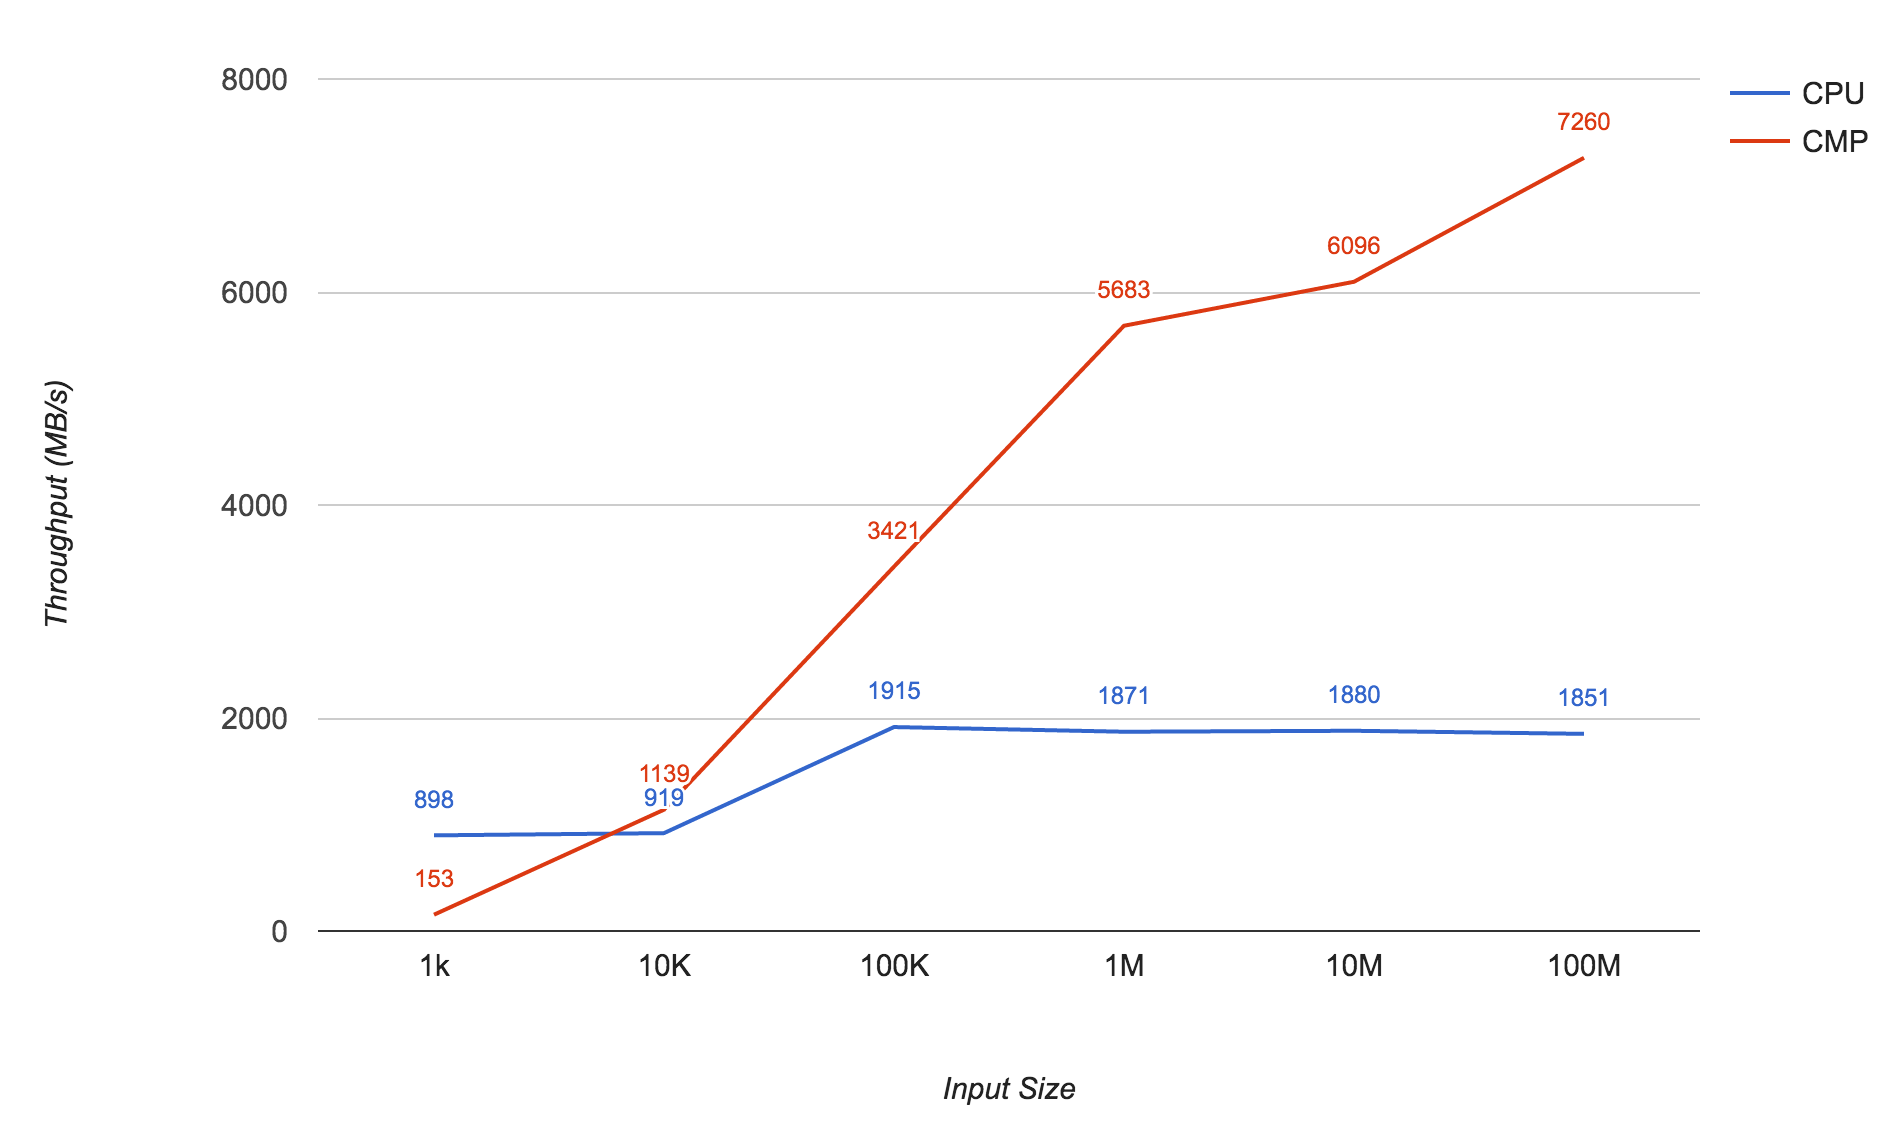
\includegraphics[width=\textwidth]{CMP.png}
    \end{center}
    \caption{{\label{fig:CMP}} CMP Merge and Sequential Merge}
    \end{figure}


